% =========================================================================== %
% Preamble                                                                    %
% =========================================================================== %

\documentclass[10pt, dvipsnames, aspectratio=169]{beamer}
%\documentclass[12pt, dipsnames, notes=only]{beamer}

\usepackage[utf8]{inputenc}
\usepackage{beamerthemesimple}

\date{February 10$^{th}$, 2021}
\title{Spectre Attacks}
\author{William Findlay}
\institute{Carleton University\\\href{mailto:will@ccsl.carleton.ca}{\ttfamily will@ccsl.carleton.ca}}

\usepackage{csquotes}
\usepackage{booktabs}

% Center floats by default
\makeatletter
\g@addto@macro\@floatboxreset{\centering}
\makeatother

\usepackage{listings}

\lstnewenvironment{listing}[1][]{\lstset{#1}}{}

\definecolor[named]{blue}{HTML}{0071b2}
\definecolor[named]{orange}{HTML}{e59c00}
\definecolor[named]{green}{HTML}{009e73}
\definecolor[named]{purple}{HTML}{88498f}
\definecolor[named]{dark-grey}{HTML}{515151}
\definecolor[named]{grey}{HTML}{797979}

\colorlet{listing-basic}{dark-grey}
\colorlet{listing-keyword}{blue}
\colorlet{listing-keyword-2}{orange}
\colorlet{listing-keyword-3}{purple}
\colorlet{listing-comment}{grey}
\colorlet{listing-string}{green}

% Set default listings style
\lstdefinestyle{listingstyle}{
    basicstyle       = {\ttfamily\color{listing-basic}\lst@ifdisplaystyle\scriptsize\fi},
    keywordstyle     = {\color{listing-keyword}\bfseries},
    keywordstyle     = {[2]\color{listing-keyword-2}\bfseries},
    keywordstyle     = {[3]\color{listing-keyword-3}\bfseries},
    identifierstyle  = {\color{listing-keyword-3}\bfseries},
    sensitive        = true,
    commentstyle     = {\color{listing-comment}},
    stringstyle      = {\color{listing-string}},
    showstringspaces = false,
    columns          = fullflexible,
    keepspaces       = true,
    literate         = {~}{$\sim$}{1},
    escapeinside     = {!@}{@!}
}
\lstset{style=listingstyle}
\lstdefinelanguage
   {x64}     % add a "x64" dialect of Assembler
   [x86masm]{Assembler} % based on the "x86masm" dialect
   % with these extra keywords:
   {morekeywords={cdqe,cqo,cmpsq,cmpxchg16b,jrcxz,lodsq,movsxd, %
                  popfq,pushfq,scasq,stosq,iretq,rdtscp,swapgs, %
                  leaq,movq,movl, %
                  rax,rdx,rcx,rbx,rsi,rdi,rsp,rbp,rip, %
                  r8,r8d,r8w,r8b,r9,r9d,r9w,r9b, %
                  r10,r10d,r10w,r10b,r11,r11d,r11w,r11b, %
                  r12,r12d,r12w,r12b,r13,r13d,r13w,r13b, %
                  r14,r14d,r14w,r14b,r15,r15d,r15w,r15b}} % etc.

\setbeamertemplate{section in toc}[sections numbered]

\hypersetup{
    colorlinks = true,
    linkcolor  = .,
    urlcolor   = blue,
    citecolor  = blue,
}
\urlstyle{tt}

\newcommand{\fullframegraphic}[1]{%
    {%
        \setwatermark{}
        \usebackgroundtemplate{\includegraphics[width=\paperwidth]{#1}}
        \begin{frame}[plain]
        \end{frame}
    }
}

\newcommand\ufootnote[1]{%
    \begingroup
        \renewcommand\thefootnote{}\footnote{\hspace{-1.8em}#1}%
        \addtocounter{footnote}{-1}%
    \endgroup
}

% Table of Contents for sections
\AtBeginSection[]
{
    \begin{frame}[c, noframenumbering, plain]
        \begin{center}
        \fontsize{42.99}{51.59} \selectfont \bfseries \color{destacado} \insertsection
        \end{center}
    \end{frame}
}

\usepackage{biblatex}
\bibliography{refs.bib}
\renewcommand*{\bibfont}{\footnotesize}

\PassOptionsToPackage{hyphens}{url}
%\setcounter{biburllcpenalty}{1}
%\setcounter{biburlucpenalty}{1}
%\setcounter{biburlbigbreakpenalty}{2}
%\setcounter{biburlbreakpenalty}{1}

\usepackage{appendixnumberbeamer}

\makeatletter
\g@addto@macro{\UrlNoBreaks}{\do:}
\g@addto@macro{\UrlBreaks}{\do\/}
\makeatother

\newenvironment{nscenter}
 {\parskip=0pt\par\nopagebreak\centering}
 {\par\noindent\ignorespacesafterend}

\let\lsi\lstinline
\newcommand{\code}[1]{\lsi[language=c]|#1|}

\usepackage{svg}

% =========================================================================== %
% Document                                                                    %
% =========================================================================== %

\begin{document}

% Optional watermark
\setwatermark[hoffset=0.3cm, voffset=0.3cm]{
\includegraphics[width=6cm]{figs/logos/spectre.png}}

% Title page
\begin{frame}[noframenumbering, plain]
  \titlepage
  \vfill
  \vspace{4em}
  {\footnotesize COMP5900X Discussion Lead}
\end{frame}

%\begin{frame}[c, noframenumbering, plain]{Outline of this Talk}
%    \tableofcontents
%\end{frame}
%
%\section{Untitled Section}

\begingroup
\setwatermark{}
\begin{frame}[c]{Spectre Overview}

\begin{columns}
  \begin{column}{0.5\textwidth}
    \begin{itemize}
      \item Spectre attacks exploit {\bf branch prediction} in modern CPUs
      \vspace{2.2em}
      \item Attacker tricks the processor into executing an {\bf incorrect branch}
      \vspace{2.2em}
      \item Instructions {\bf leak information} into the $\mu$-architecture (e.g.~the cache)
      \vspace{2.2em}
      \item Attacker can {\bf recover the information} using a number of {\bf $\boldsymbol{\mu}$-architectural side channels}
    \end{itemize}
  \end{column}

  \begin{column}{0.5\textwidth}
    \color{black}
    \centering
    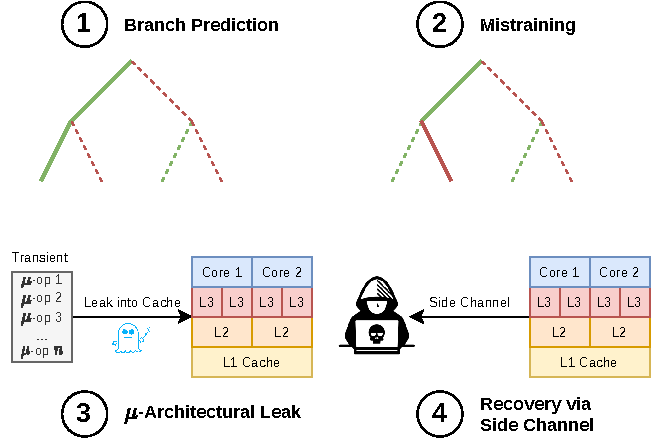
\includegraphics[width=0.8\linewidth]{figs/overview.pdf}
  \end{column}
\end{columns}
\end{frame}
\endgroup

\begin{frame}[c]{Goals}
  \begin{enumerate}
    \item Provide an overview of Spectre attacks
    \vfill
    \item Differentiate Spectre from Meltdown (variant 3)
    \vfill
    \item Present proof of concept exploits for Spectre variant 1 and 2
    \vfill
    \item Evaluate the practical performance/risks associated with Spectre attacks
    \vfill
    \item Present future avenues for Spectre exploitation (variant 4, other side channels)
    \vfill
    \item Discuss and propose mitigations against current/future Spectre attacks
  \end{enumerate}
\end{frame}

\begin{frame}[c]{Threat Model and Assumptions}
  \begin{itemize}
    \item Roughly similar threat model to the Meltdown paper
  \end{itemize}
\end{frame}

\begin{frame}[c]{Relevance and Impact}
  \begin{itemize}
    \item Foo
  \end{itemize}
\end{frame}

\begingroup
\setwatermark{}
\begin{frame}[c]{Spectre vs Meltdown (tl;dr)}
  \begin{columns}
    \begin{column}[t]{0.5\textwidth}
      \centering
      \includesvg[height=6em]{figs/logos/meltdown.svg}
      \begin{itemize}
        \item Dumps arbitrary kernel memory
        \begin{itemize}
          \item And thus physical memory
        \end{itemize}
        \item Victim is mapped kernel memory
        \begin{itemize}
          \item No victim process required
        \end{itemize}
        \item Mostly stopped by KPTI (KAISER) mitigation
        \item Affects only some CPUs (mostly Intel)
        \item Easier to exploit
      \end{itemize}
    \end{column}

    \begin{column}[t]{0.5\textwidth}
      \centering
      
\includegraphics[height=6em]{figs/logos/spectre.png}
      \begin{itemize}
        \item Leak secrets via speculative execution
        \item Victim is another process or the kernel
        \begin{itemize}
          \item But can also be the same process
        \end{itemize}
        \item Totally unaffected by KPTI
        \item Affects a wide range of CPUs
        \begin{itemize}
          \item Multiple vendors
        \end{itemize}
        \item Harder to exploit
      \end{itemize}
    \end{column}
  \end{columns}
\end{frame}
\endgroup

\begin{frame}[c]{Spectre Building Blocks}
  \begin{enumerate}
    \item {\bf\color{blue}Setup Phase}
    \begin{itemize}
      \item Mistrain the CPU's branch predictor
      \item Optionally: Induce speculative execution (e.g.~evict branch-specific value $n$ from the cache)
    \end{itemize}

    \vfill
    \item {\bf\color{orange}Execution Phase}
    \begin{itemize}
      \item Attacker provides some attacker-controlled value to victim (e.g.~$n = 3000000$)
      \begin{itemize}
        \item Could be via a system call, a socket, file I/O, etc.
        \item Or the victim could be our own process (much simpler)
      \end{itemize}
      \item CPU mispredicts a branch on the value of $n$
      \item Transient instructions encode a secret value $v$ (dependent on $n$) into $\mu$-architectural state
    \end{itemize}

    \vfill
    \item {\bf\color{green}Recovery Phase}
    \begin{itemize}
      \item Attacker recovers information about $v$ using a $\mu$-architectural side channel
      \item E.g.~flush+reload, evict+reload, evict+time
    \end{itemize}
  \end{enumerate}
\end{frame}

\begin{frame}[c]{Branch Prediction}
  \begin{itemize}
    \item Code branches depend on value(s) in memory
    \begin{itemize}
      \item \code{if (foo < size) \{ A(foo); \} else \{ B(foo); \}}
      \item Which path we take depends on \code{foo} and \code{size}
    \end{itemize}

    \vfill
    \item But fetching these values can be slow
    \begin{itemize}
      \item Suppose that foo is a cache hit but size is a cache miss
      \item If CPU is idle during this time, we lose out on performance
      \item Wasting clock cycles
    \end{itemize}

    \vfill
    \item So what can the CPU do?
    \begin{itemize}
      \item Make a guess and just roll with it while fetching the value
      \item If our guess is right, great! We saved some time
      \item Otherwise, roll back (\textit{retire}) erroneous state changes and execute correct code
    \end{itemize}
  \end{itemize}
\end{frame}

\fullframegraphic{figs/silly/this_is_fine.jpg}

\begin{frame}[c]{But There is One Small (Huge) Problem}{}
  {\bf Transient Instructions}
  \begin{itemize}
    \item Incorrect branch predictions are retired
    \item But $\mu$-architectural effects remain
    \item Number of transient instructions depends on the size of the CPU's reorder buffer
    \item Can be quite high in practice
  \end{itemize}

  \vfill
  {\bf Why is This a Problem?}
  \begin{itemize}
    \item Erroneous effects are encoded in $\mu$-architectural state, e.g.~cache memory
    \item This \textit{should} be totally transparent to the architectural state
    \item But attackers can transfer $\mu$-architectural state into architectural state via side channels
  \end{itemize}
  %\begin{itemize}
  %  \item An incorrect branch prediction leads to \alert{transient instructions}
  %  \begin{itemize}
  %    \item (c.f.~Meltdown from last week)
  %  \end{itemize}

  %  \vfill
  %  \item Ordinarily rolled back (\alert{retired}) by the CPU

  %  \vfill
  %  \item But these transient instructions have \alert{micro-architectural side effects}
  %  \begin{itemize}
  %    \item From the architecture's perspective, effects are rolled back
  %    \item But the \alert{cache remains affected}
  %  \end{itemize}
  %\end{itemize}
\end{frame}

\begingroup
\setwatermark{}
\begin{frame}[c]{Branch Prediction Illustrated}
  \begin{center}
    \color{black}
    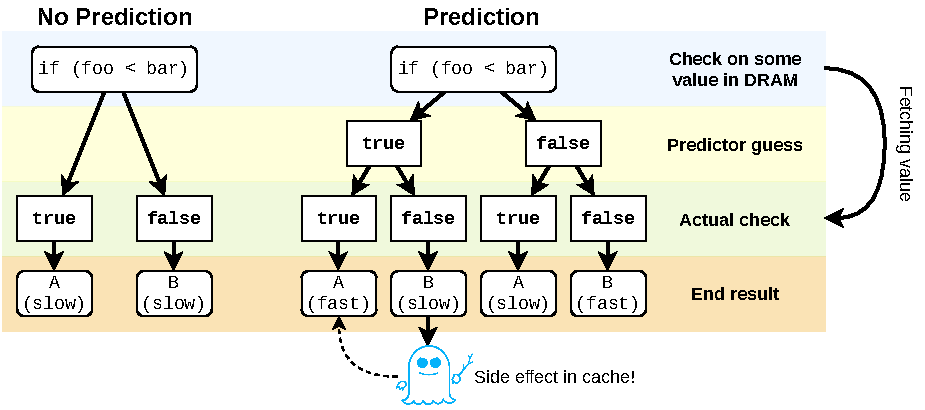
\includegraphics[width=0.9\textwidth]{figs/prediction.pdf}
  \end{center}
\end{frame}
\endgroup

\begin{frame}[c]{(Mis)Training the Branch Predictor}{}
  {\bf How to Induce Speculative Execution?}
  \begin{itemize}
    \item Dynamic branch predictors\footnote{Mittal \cite{mittal2019_branch_prediction} is a nice resource for those who want an in-depth study of branch prediction techniques} update their prediction model using historical data
    \item The attacker can invoke a specific branch target
    \begin{itemize}
      \item E.g.~Use a \code{foo} such that \code{foo < size}
      \item Number of times they need to do this depends on BP implementation
    \end{itemize}
  \end{itemize}

  \vfill
  {\bf After Mistraining}
  \begin{itemize}
    \item Attacker can supply an out-of-bounds \code{foo}
    \begin{itemize}
      \item But the branch predictor will still execute as if \code{foo < size}
      \item Transient code accesses some secret at an offset computed using \code{foo}
      \item That secret leaks into cache memory
    \end{itemize}
  \end{itemize}
\end{frame}

\begin{frame}[c]{Cache-Based Side Channels}
  \begin{itemize}
    \item The Spectre paper primarily focuses on cache-based side channels

    TODO Finish this

    \vfill
    \item The authors note that Spectre variants could exploit arbitrary observable effects of transient code
    \begin{itemize}
      \item Contention for resources (buses, arithmetic units, etc.)
      \item
    \end{itemize}
  \end{itemize}
\end{frame}

\begin{frame}[c,fragile]{Direct and Indirect Branching}
  \begin{columns}
    \begin{column}[t]{0.5\textwidth}
      {\bf\color{blue}\Large Direct Branches}
      \begin{itemize}
        \item Conditionals, jumps, etc.
        \item Prediction may not match check
        \begin{itemize}
          \item Spectre variant 1
        \end{itemize}
      \end{itemize}

      \vspace{1em}
      \begin{listing}[language=c,gobble=8,xleftmargin=5em]
        int x;
        int arr[256];

        /* ... */

        if (foo < 256) {
            x = arr[foo];
        }
      \end{listing}
    \end{column}

    \begin{column}[t]{0.5\textwidth}
      {\bf\color{orange}\Large Indirect Branches}
      \begin{itemize}
        \item Call based on function pointer (address)
        \item Predictor can guess an incorrect address
        \begin{itemize}
          \item Spectre variant 2
        \end{itemize}
      \end{itemize}

      \vspace{1em}
      \begin{listing}[language=c,gobble=8,xleftmargin=5em]
        int my_fn(int foo) {
            return foo * foo;
        }

        /* ... */

        int (*fn_ptr)(int) = &my_fn;
        fn_ptr(42);
      \end{listing}
      %{\footnotesize Results in:}
      %\begin{listing}[language=x64,gobble=8]
      %  ; ...
      %  leaq	my_fn(%rip), %rax
      %  movq	%rax, -8(%rbp)
      %  movq	-8(%rbp), %rax
      %  movl	$42, %edi
      %  call	*%rax
      %  ; ...
      %\end{listing}
    \end{column}
  \end{columns}
\end{frame}

\begin{frame}[c]{Spectre Variants}
  \begin{itemize}
    \item Foo
  \end{itemize}
\end{frame}

\begin{frame}[c]{Evaluation}
  \begin{itemize}
    \item Foo
  \end{itemize}
\end{frame}

\begin{frame}[c]{Mitigating Variant 1}
  \begin{itemize}
    \item Foo
  \end{itemize}
\end{frame}

\begin{frame}[c]{Mitigating Variant 2}
  \begin{itemize}
    \item Foo
  \end{itemize}
\end{frame}

\begin{frame}[c]{Other Mitigation Strategies}
  \begin{itemize}
    \item Foo
  \end{itemize}
\end{frame}

\begin{frame}[c]{Discussion}
  \begin{itemize}
    \item Foo
  \end{itemize}
\end{frame}

\appendix

\nocite{*}
\begin{frame}[allowframebreaks, noframenumbering, plain]
  \frametitle{References}
  \sloppy
  \printbibliography
\end{frame}

\end{document}

% vim:syn=tex

